\documentclass[11pt,aspectratio=43]{beamer}

\usepackage{amsmath,amssymb}
\usepackage{array}
\usepackage{booktabs}
\usepackage{graphicx}
\usepackage[numbers,sort&compress]{natbib}
\usepackage{tikz}
\usepackage{xcolor}
\usetikzlibrary{arrows.meta,calc,positioning,shapes.geometric}

\definecolor{accent}{HTML}{2E75B6}

\setbeameroption{hide notes}
\setbeamertemplate{navigation symbols}{}
\setbeamersize{text margin left=0.8cm,text margin right=0.8cm}

\setbeamercolor{normal text}{fg=black,bg=white}
\setbeamercolor{frametitle}{fg=black,bg=white}
\setbeamercolor{title}{fg=black}
\setbeamercolor{structure}{fg=black}
\setbeamercolor{alerted text}{fg=accent}
\setbeamercolor{block title}{fg=black,bg=black!10}
\setbeamercolor{block body}{fg=black,bg=black!3}
\setbeamercolor{itemize item}{fg=black}
\setbeamercolor{itemize subitem}{fg=black}

\setbeamerfont{title}{size=\normalsize,series=\bfseries}
\setbeamerfont{frametitle}{size=\normalsize,series=\bfseries}
\setbeamerfont{block title}{size=\normalsize,series=\bfseries}
\setbeamerfont{block body}{size=\normalsize}

\setbeamertemplate{footline}{%
  \leavevmode%
  \hbox{%
    \begin{beamercolorbox}[wd=\paperwidth,ht=2.8ex,dp=1.2ex,rightskip=0.8cm]{author in head/foot}%
      \insertframenumber
    \end{beamercolorbox}%
  }%
}

\newcommand{\figorplaceholder}[2]{%
  \IfFileExists{#1}{%
    \includegraphics[width=\linewidth,height=#2,keepaspectratio]{#1}%
  }{%
    \fbox{\parbox[c][#2][c]{0.92\linewidth}{\centering Missing figure:\\\texttt{\detokenize{#1}}}}%
  }%
}

\newcommand{\preliminarytag}{%
  \colorbox{accent!12}{\textcolor{accent}{\textbf{\strut Preliminary}}}%
}

\title{Optimising the RL Policy for Octopus CXL Memory Pooling}
\author{Pulak Mehrotra}
\date{March 2026}

\begin{document}

\begin{frame}[plain]
  \titlepage
\end{frame}

\begin{frame}{Recap: Octopus topology makes the allocation problem structurally hard.}
  \begin{columns}[T,onlytextwidth]
    \column{0.52\textwidth}
      \centering
      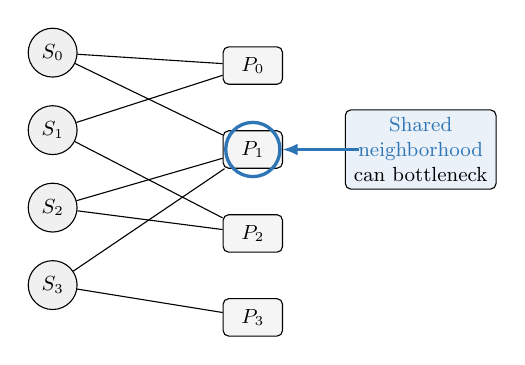
\begin{tikzpicture}[
          scale=0.82,
          transform shape,
          every node/.style={font=\small},
          host/.style={draw, circle, fill=black!6, minimum size=0.72cm},
          mpd/.style={draw, rounded corners=2pt, fill=black!4, minimum width=0.92cm, minimum height=0.58cm},
          callout/.style={draw, rounded corners=2pt, fill=accent!10, text width=2.1cm, align=center, minimum height=0.7cm}
      ]
        \node[host] (h0) at (0,2.2) {$S_0$};
        \node[host] (h1) at (0,1.0) {$S_1$};
        \node[host] (h2) at (0,-0.2) {$S_2$};
        \node[host] (h3) at (0,-1.4) {$S_3$};

        \node[mpd] (p0) at (3.1,2.0) {$P_0$};
        \node[mpd] (p1) at (3.1,0.7) {$P_1$};
        \node[mpd] (p2) at (3.1,-0.6) {$P_2$};
        \node[mpd] (p3) at (3.1,-1.9) {$P_3$};

        \draw (h0) -- (p0);
        \draw (h0) -- (p1);
        \draw (h1) -- (p0);
        \draw (h1) -- (p2);
        \draw (h2) -- (p1);
        \draw (h2) -- (p2);
        \draw (h3) -- (p1);
        \draw (h3) -- (p3);

        \draw[accent, line width=1.2pt] ($(p1)+(-0.42,0)$) arc (180:540:0.42);
        \node[callout] at (5.7,0.7) {\textcolor{accent}{Shared neighborhood}\\can bottleneck};
        \draw[-{Latex[length=2mm]},accent,line width=1.1pt] (4.75,0.7) -- (3.55,0.7);
      \end{tikzpicture}
    \column{0.48\textwidth}
      \begin{itemize}
        \item Each VM arrival can use only the host's reachable MPDs.
        \item Multiple servers can collide on the same small MPD neighborhood.
        \item There is no cheap migration loop to repair a bad early placement.
        \item The real objective is the worst MPD peak, not average load.
      \end{itemize}

      \vspace{0.4em}
      Provisioning is set by the hottest MPD.
  \end{columns}
\end{frame}

\begin{frame}{The current implementation already evaluates capacity outcomes across randomized pod mappings.}
  \begin{columns}[T,onlytextwidth]
    \column{0.52\textwidth}
      \centering
      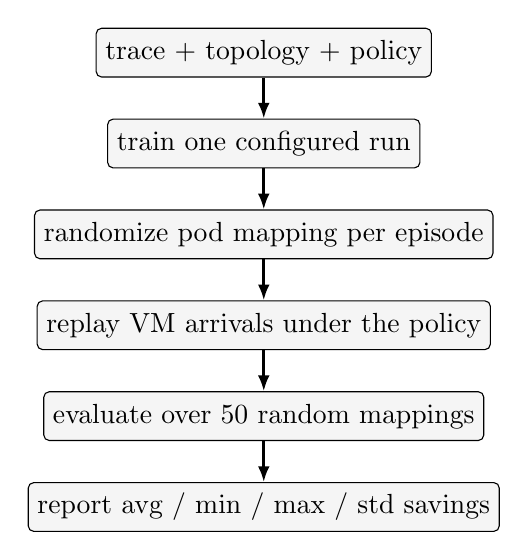
\begin{tikzpicture}[
          node distance=0.52cm,
          box/.style={draw, rounded corners=2pt, minimum width=3.8cm, minimum height=0.62cm, align=center, fill=black!4},
          arr/.style={-{Latex[length=2mm]}, line width=0.95pt}
      ]
        \node[box] (trace) {trace + topology + policy};
        \node[box, below=of trace] (train) {train one configured run};
        \node[box, below=of train] (remap) {randomize pod mapping per episode};
        \node[box, below=of remap] (replay) {replay VM arrivals under the policy};
        \node[box, below=of replay] (eval) {evaluate over 50 random mappings};
        \node[box, below=of eval] (report) {report avg / min / max / std savings};
        \draw[arr] (trace) -- (train);
        \draw[arr] (train) -- (remap);
        \draw[arr] (remap) -- (replay);
        \draw[arr] (replay) -- (eval);
        \draw[arr] (eval) -- (report);
      \end{tikzpicture}
    \column{0.48\textwidth}
      \begin{itemize}
        \item The code path is not scoring a single cherry-picked topology.
        \item Training is still simple: one trace and one configured topology per run.
        \item Evaluation already reports a distribution over randomized mappings.
        \item The metric to trust is pooling savings or required per-MPD capacity, not raw RL reward.
      \end{itemize}
  \end{columns}
\end{frame}

\begin{frame}{The current SAC policy collapses load onto a few MPDs.}
  \begin{flushright}
    \preliminarytag
  \end{flushright}
  \begin{columns}[T,onlytextwidth]
    \column{0.5\textwidth}
      \figorplaceholder{../../v1/figs/mhd_timeseries_greedy.png}{0.56\textheight}

      \centering Greedy
    \column{0.5\textwidth}
      \figorplaceholder{../../v1/figs/mhd_timeseries_rl.png}{0.56\textheight}

      \centering Current SAC
  \end{columns}

  \vspace{0.4em}
  \begin{itemize}
    \item The clearest current failure signal is about a 20x max/min MPD imbalance.
    \item Behaviorally, the policy is not yet acting like a load balancer, which is a stronger diagnosis than ``reward is noisy''.
    \item This is the evidence that motivates changing the task formulation before changing the deployment story.
  \end{itemize}
\end{frame}

\begin{frame}{1M samples with fast config yields $\sim$62k policy updates and no meaningful policy difference.}
  \begin{columns}[T,onlytextwidth]
    \column{0.52\textwidth}
      \centering
      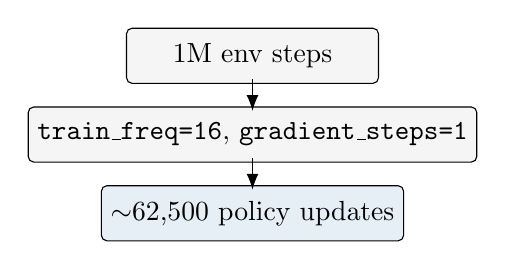
\begin{tikzpicture}[
          x=1cm, y=1cm,
          lbl/.style={font=\scriptsize},
          box/.style={draw, rounded corners=2pt, fill=black!4, minimum width=3.2cm, minimum height=0.7cm, align=center}
      ]
        \node[box] at (2.5,2.5) {1M env steps};
        \node[box] at (2.5,1.5) {\texttt{train\_freq=16}, \texttt{gradient\_steps=1}};
        \node[box, fill=accent!12] at (2.5,0.5) {$\sim$62,500 policy updates};
        \draw[-{Latex[length=2mm]}] (2.5,2.2) -- (2.5,1.8);
        \draw[-{Latex[length=2mm]}] (2.5,1.2) -- (2.5,0.8);
      \end{tikzpicture}
    \column{0.48\textwidth}
      \begin{itemize}
        \item Standard vs fast config: \textbf{no meaningful difference} in policy quality.
        \item Policy optimized fairly quickly---converged within 62k updates.
        \item \alert{Takeaway:} the bottleneck is not training volume; it is state and reward design.
      \end{itemize}
  \end{columns}
\end{frame}

\begin{frame}{What I'm drilling down on: three fixes.}
  \centering
  \begin{enumerate}
    \item \textbf{State} --- expose future pressure, not just current load
    \item \textbf{Reward} --- score balanced low load, not only the current peak
    \item \textbf{Learning methodology} --- learnability first, then algorithm choice
  \end{enumerate}
  \vspace{0.8em}
  \raggedright
  The next slides spell out each fix.
\end{frame}

\begin{frame}{Fix 1: The state should expose future pressure instead of only current load.}
  \centering
  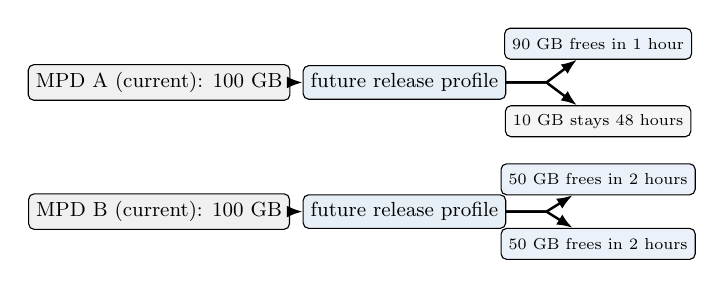
\begin{tikzpicture}[
      scale=0.82,
      transform shape,
      stage/.style={draw, rounded corners=2pt, minimum height=0.52cm, minimum width=2.2cm, align=center, fill=black!6, font=\small},
      profile/.style={draw, rounded corners=2pt, minimum height=0.52cm, minimum width=2.4cm, align=center, fill=accent!12, font=\small},
      release/.style={draw, rounded corners=2pt, minimum height=0.48cm, minimum width=2.1cm, align=center, fill=accent!10, font=\scriptsize},
      sticky/.style={draw, rounded corners=2pt, minimum height=0.48cm, minimum width=2.1cm, align=center, fill=black!4, font=\scriptsize},
      arr/.style={-{Latex[length=2mm]}, line width=0.9pt}
  ]
    % MPD A
    \node[stage] (aCurr) at (-0.6,3.0) {MPD A (current): $100$ GB};
    \node[profile] (aProf) at (3.2,3.0) {future release profile};
    \node[release] (a90) at (6.2,3.6) {90 GB frees in 1 hour};
    \node[sticky] (a10) at (6.2,2.4) {10 GB stays 48 hours};
    \draw[arr] (aCurr) -- (aProf);
    \draw[arr] (aProf) -- (5.4,3.0) -- (a90);
    \draw[arr] (aProf) -- (5.4,3.0) -- (a10);

    % MPD B
    \node[stage] (bCurr) at (-0.6,1.0) {MPD B (current): $100$ GB};
    \node[profile] (bProf) at (3.2,1.0) {future release profile};
    \node[release] (b50a) at (6.2,1.5) {50 GB frees in 2 hours};
    \node[release] (b50b) at (6.2,0.5) {50 GB frees in 2 hours};
    \draw[arr] (bCurr) -- (bProf);
    \draw[arr] (bProf) -- (5.4,1.0) -- (b50a);
    \draw[arr] (bProf) -- (5.4,1.0) -- (b50b);
  \end{tikzpicture}

  \vspace{0.6em}
  \raggedright
  \begin{itemize}
    \item The current state mostly treats each MPD as a single instantaneous load number.
    \item Two MPDs can look identical now while having very different near-future headroom.
    \item \alert{Design principle:} represent how much memory comes back and when it comes back.
  \end{itemize}
\end{frame}

\begin{frame}{The proposed state adds future-pressure features per reachable MPD.}
  \begin{columns}[T,onlytextwidth]
    \column{0.48\textwidth}
      \begin{block}{Current state (unchanged)}
        \begin{itemize}
          \item Reachable MPD loads $c_j$
          \item Connectivity mask
          \item Incoming VM size
          \item Global peak load
          \item Hour-of-day encoding
        \end{itemize}
      \end{block}
    \column{0.52\textwidth}
      \begin{block}{Added or changed}
        \begin{itemize}
          \item \textbf{Short-horizon release}: memory expected to free in next 1--2 hours
          \item \textbf{Medium-horizon release}: memory expected to free in 2--24 hours
          \item \textbf{Sticky load}: memory expected to stay beyond 24 hours
          \item \textbf{VM count} per reachable MPD
        \end{itemize}
      \end{block}
  \end{columns}
  \vspace{0.2em}
  \small
  \textbf{Temporal data:} Diagram maps to buckets---short (1--2 hr), medium (2--24 hr), sticky ($>$24 hr). MPD A: 90$\rightarrow$short, 10$\rightarrow$sticky. MPD B: 100$\rightarrow$medium. These features distinguish MPDs that look identical by current load alone.
\end{frame}

\begin{frame}{Fix 2: The reward should score balanced low load instead of only the current peak.}
  \begin{columns}[T,onlytextwidth]
    \column{0.48\textwidth}
      \centering
      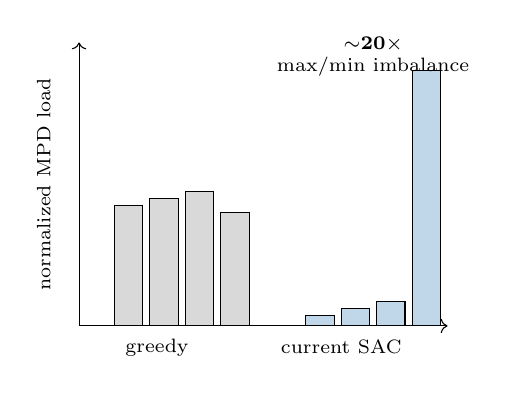
\begin{tikzpicture}[
          x=0.9cm, y=0.9cm,
          lbl/.style={font=\scriptsize},
          bar1/.style={draw, fill=black!15},
          bar2/.style={draw, fill=accent!30}
      ]
        \draw[->] (0,0) -- (0,4.0);
        \draw[->] (0,0) -- (5.2,0);
        \node[lbl, rotate=90] at (-0.5,2.0) {normalized MPD load};
        \node[lbl] at (1.1,-0.3) {greedy};
        \node[lbl] at (3.7,-0.3) {current SAC};
        \draw[bar1] (0.5,0) rectangle (0.9,1.7);
        \draw[bar1] (1.0,0) rectangle (1.4,1.8);
        \draw[bar1] (1.5,0) rectangle (1.9,1.9);
        \draw[bar1] (2.0,0) rectangle (2.4,1.6);
        \draw[bar2] (3.2,0) rectangle (3.6,0.15);
        \draw[bar2] (3.7,0) rectangle (4.1,0.25);
        \draw[bar2] (4.2,0) rectangle (4.6,0.35);
        \draw[bar2] (4.7,0) rectangle (5.1,3.6);
        \node[lbl, align=center] at (4.15,3.8) {\textbf{$\sim$20$\times$}\\max/min imbalance};
      \end{tikzpicture}
    \column{0.52\textwidth}
      \begin{itemize}
        \item The reward is \textbf{sparse}: most signal comes from whichever MPD is currently worst.
        \item Bad choices among non-peak MPDs can look nearly identical---no gradient to balance load.
        \item Diagnostics point to reward design as a major contributor to load collapse.
      \end{itemize}
      \vspace{0.3em}
      \alert{Next:} propose a denser reward.
  \end{columns}
\end{frame}

\begin{frame}{Why the current reward is the problem.}
  \begin{columns}[T,onlytextwidth]
      \column{0.48\textwidth}
        \begin{block}{Current immediate reward}
          \[
          r_t \propto -\Delta \max_j c_j(t)
          \]
          \begin{itemize}
            \item Most of the signal comes from whichever MPD is currently worst.
            \item Bad choices among non-peak MPDs can look nearly identical.
          \end{itemize}
        \end{block}
      \column{0.52\textwidth}
        \begin{block}{Proposed immediate reward}
          \[
          \begin{aligned}
          R_t ={}& \alpha \,\text{Peak}(t) \\
                &- \beta \,\mathrm{Var}(c(t)) \\
                &- \gamma \,\text{OverCap}(t)
          \end{aligned}
          \]
          \begin{itemize}
            \item The peak term keeps the reward aligned with required capacity.
            \item The variance term gives dense feedback across all MPDs.
            \item The over-cap term keeps capacity violations explicit.
          \end{itemize}
      \end{block}
  \end{columns}
\end{frame}

\begin{frame}{Fix 3: The current bottleneck is learnability rather than catastrophic forgetting.}
  \centering
  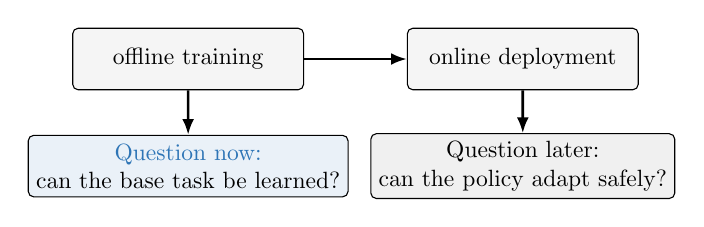
\begin{tikzpicture}[
      scale=0.85,
      transform shape,
      stage/.style={draw, rounded corners=2pt, minimum width=3.45cm, minimum height=0.92cm, align=center, fill=black!4},
      note/.style={draw, rounded corners=2pt, minimum width=3.75cm, minimum height=0.92cm, align=center},
      arr/.style={-{Latex[length=2mm]}, line width=0.95pt}
  ]
    \node[stage] (offline) at (2.0,2.1) {offline training};
    \node[stage] (deploy) at (7.0,2.1) {online deployment};
    \node[note, fill=accent!10] (learn) at (2.0,0.5) {\textcolor{accent}{Question now:}\\can the base task be learned?};
    \node[note, fill=black!6] (forget) at (7.0,0.5) {Question later:\\can the policy adapt safely?};
    \draw[arr] (offline) -- (deploy);
    \draw[arr] (offline) -- (learn);
    \draw[arr] (deploy) -- (forget);
  \end{tikzpicture}

  \vspace{0.8em}
  \raggedright
  \begin{itemize}
    \item The present failure appears during offline training, before any deployment drift.
    \item That makes state, reward, and training protocol the immediate issues.
    \item Same framing as robotics: learn the task in sim first; adaptation to real-world drift comes later.
  \end{itemize}
\end{frame}

\begin{frame}{The next round should separate learnability claims from generalization claims cleanly.}
  \begin{columns}[T,onlytextwidth]
    \column{0.52\textwidth}
      \centering
      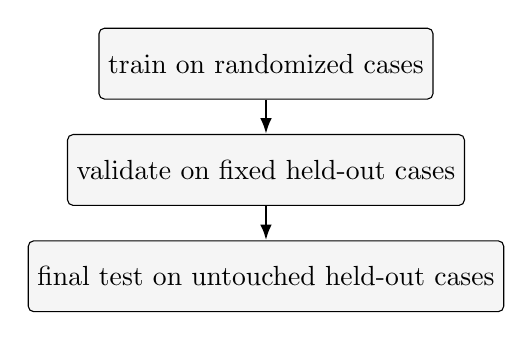
\begin{tikzpicture}[
          phase/.style={draw, rounded corners=2pt, minimum width=3.7cm, minimum height=0.9cm, align=center, fill=black!4},
          arr/.style={-{Latex[length=2mm]}, line width=0.95pt}
      ]
        \node[phase] (train) at (2.3,2.8) {train on randomized cases};
        \node[phase] (val) at (2.3,1.45) {validate on fixed held-out cases};
        \node[phase] (test) at (2.3,0.1) {final test on untouched held-out cases};
        \draw[arr] (train) -- (val);
        \draw[arr] (val) -- (test);
      \end{tikzpicture}
    \column{0.48\textwidth}
      \begin{itemize}
        \item Randomize traces, time windows, pod mappings, and CXL fractions during training.
        \item Use validation to select checkpoints, not final test traces.
        \item Keep the final test set untouched until the end.
        \item Run ablations in this order: state, reward, training, then algorithm.
      \end{itemize}
  \end{columns}
  \alert{First success criterion:} beat greedy on held-out offline cases.
\end{frame}

\begin{frame}{SAC: off-policy actor-critic with entropy regularization.}
  \begin{block}{What it is}
    Soft Actor-Critic \cite{haarnoja2018sac} maximizes expected return plus policy entropy. It uses a replay buffer and learns from off-policy data, making it sample-efficient for continuous actions.
  \end{block}
  \vspace{0.4em}
  \textbf{Why it matters for Octopus:} SAC is our current baseline. Its continuous action space fits the allocation-split problem. The replay buffer can mix data from different topologies and traces---which helps sample efficiency but may hurt generalization if the mix is wrong.
\end{frame}

\begin{frame}{PPO: on-policy policy gradient with a clipped objective.}
  \begin{block}{What it is}
    Proximal Policy Optimization \cite{schulman2017ppo} updates the policy using only on-policy data and clips the probability ratio to limit step size. No replay buffer.
  \end{block}
  \vspace{0.4em}
  \textbf{Why it matters for Octopus:} PPO is the clean control to test whether the base task is learnable. If PPO fails where SAC fails, the problem is likely state or reward design, not replay-buffer effects.
\end{frame}

\begin{frame}{LCPO: online adaptation without catastrophic forgetting.}
  \begin{block}{What it is}
    LCPO \cite{hamadanian2025lcpo} adapts the policy online in non-stationary, context-driven environments. It constrains updates to preserve behavior on recent context while adapting to new regimes.
  \end{block}
  \vspace{0.4em}
  \textbf{Why it matters for Octopus:} LCPO addresses deployment-time drift (e.g., new datacenter, workload shift). It does not fix an unlearnable offline task---use it only after an offline policy already beats greedy.
\end{frame}

\begin{frame}{Algorithm choice should follow evidence from SAC to PPO to LCPO.}
  \begin{columns}[T,onlytextwidth]
    \column{0.50\textwidth}
      \begin{block}{Offline learnability}
        \begin{itemize}
          \item SAC stays as the current continuous-action baseline.
          \item PPO is the clean next control because it removes replay-buffer mixing and tests whether an on-policy learner can solve the base task.
          \item If PPO still fails, the right conclusion is that task formulation is still wrong.
        \end{itemize}
      \end{block}
    \column{0.50\textwidth}
      \begin{block}{Online adaptation}
        \begin{itemize}
          \item LCPO is the deployment-time method for non-stationary contexts.
          \item Its value is forgetting resistance, not fixing an unlearnable offline task.
          \item It should enter only after offline policies already beat greedy consistently.
        \end{itemize}
      \end{block}
  \end{columns}

  \vspace{0.3em}
  \alert{Decision rule:} if PPO does not work after state, reward, and training fixes, do not jump to LCPO.
\end{frame}

\begin{frame}{The next milestone is a credible offline result that beats greedy on held-out cases.}
  \begin{itemize}
    \item Finish the state and reward redesign, then rerun offline training with a larger budget and cleaner train/validation/test separation.
    \item Add learning evidence: training/validation curves that show whether the policy is actually learning (not just a final checkpoint).
    \item Report four quantities together: pooling savings, MPD imbalance, oversubscribed MPDs, and variance across randomized pod mappings.
    \item Use PPO as the immediate control once the measurement path is clean enough to compare against SAC.
    \item Defer LCPO and other online machinery until there is one offline result that looks trustworthy to a systems audience.
  \end{itemize}
\end{frame}

\begin{frame}{Advisor feedback on the experimental scope and decision rule would be most useful now.}
  \begin{block}{Questions for feedback}
    \begin{enumerate}
      \item Is ``beat greedy on held-out offline cases'' the right near-term bar before any online adaptation work?
      \item Is the proposed order of ablations correct: 1. state, 2. reward, 3. training protocol and algorithm?
      \item Can we get more data here?
    \end{enumerate}
    \vspace{0.2em}
    \scriptsize
    \textbf{Stakes:} (1)~Success criterion for next phase. (2)~Order isolates causes. (3)~10 traces may suffice for train/val/test; need to know before scaling up.
  \end{block}

  \vspace{0.4em}
  \end{frame}

\begin{frame}[allowframebreaks]{References}
  \bibliographystyle{ieeetr}
  \bibliography{../../v1/references}
\end{frame}

\begin{frame}{Milestones dashboard (what I will bring next).}
  \scriptsize
  \begin{tabular}{p{0.22\linewidth}p{0.43\linewidth}p{0.30\linewidth}}
    \toprule
    \textbf{Milestone} & \textbf{What I will do} & \textbf{What I will show} \\
    \midrule
    Fix 1: state &
    Add future-pressure features per reachable MPD (short / medium / sticky + VM count) &
    State-ablation table: load-only vs +pressure; savings + imbalance + over-cap \\
    Fix 2: reward &
    Replace peak-only proxy with denser immediate reward (peak + variance + explicit over-cap) &
    Reward-ablation table + one failure-analysis plot (per-MPD load timeline) \\
    Fix 3: learning methodology &
    Clean train/val/test separation; larger offline budget; disciplined reporting &
    Learning evidence: train/val curves + held-out savings (not just a final checkpoint) \\
    Systems reporting &
    Report metrics together across randomized pod mappings &
    One result table: pooling savings, MPD imbalance, oversubscribed MPDs, variance \\
    Scope gate &
    Defer online adaptation machinery until one offline result is credible &
    Clear stop/go: offline beats greedy on held-out cases before LCPO \\
    \bottomrule
  \end{tabular}
\end{frame}

\end{document}
